% ----------------------------------------------------------
% Document class
% ----------------------------------------------------------
\documentclass[letterpaper]{article}

% ----------------------------------------------------------
% Packages
% ----------------------------------------------------------
\usepackage{geometry}
\usepackage{xcolor}
\usepackage{amsmath}
\usepackage{amssymb}
\usepackage{amsthm}
\usepackage[some]{background}
\usepackage{lipsum}
\usepackage{microtype}

% Uncomment this line to compile with pdflatex
\def\pdflatex{}

\ifdefined \pdflatex % we are running pdflatex, so convert .eps files to .pdf
\usepackage{graphicx}
\usepackage{epstopdf}
\epstopdfsetup{update}
\pdfobjcompresslevel=0
\pdfminorversion=5
\pdfinfo{
	/Title (Preliminary Concept)
	/Author (Stiven S. Dias)
	/Subject ()
	/Keywords ()
	/GTS_PDFXVersion (PDF/X-3:2002)
}
\else % we are running LaTeX, not pdflatex
\usepackage[dvips]{graphicx}
\usepackage{graphicx}
\fi

% ----------------------------------------------------------
% Definitions
% ----------------------------------------------------------
\definecolor{titlepagecolor}{cmyk}{1,.60,0,.40}

\backgroundsetup{
scale=1,
angle=0,
opacity=1,
contents={\begin{tikzpicture}[remember picture,overlay]
 \path [fill=titlepagecolor] (current page.west)rectangle (current page.north east); 
 \draw [color=white, very thick] (5,0)--(5,0.5\paperheight);
\end{tikzpicture}}
}

\makeatletter                   
\def\printauthor{%                  
    {\large \@author}}          
\makeatother

% ----------------------------------------------------------
% Authors
% ----------------------------------------------------------
\author{%
    Stiven S. Dias \\
    Instituto Tecnol\'ogico de Aeron\'autica\\
    \texttt{stivendias@gmail.com}\vspace{40pt}
}

% ----------------------------------------------------------
% Begin document
% ----------------------------------------------------------
\begin{document}

% ----------------------------------------------------------
% Title page
% ----------------------------------------------------------
\begin{titlepage}
\BgThispage
\newgeometry{left=1cm,right=6cm,bottom=2cm}
\vspace*{0.3\textheight}
\noindent
\textcolor{white}{\Huge\textbf{\textsf{Detection and Tracking of Moving Objects}}}
\vspace*{2cm}\par
\noindent
\begin{minipage}{0.35\linewidth}
    \begin{flushright}
        \printauthor
    \end{flushright}
\end{minipage} \hspace{15pt}
%
\begin{minipage}{0.02\linewidth}
    \rule{1pt}{175pt}
\end{minipage} \hspace{-10pt}
%
\begin{minipage}{0.63\linewidth}
\vspace{5pt}

% ----------------------------------------------------------
% Abstract
% ----------------------------------------------------------

\begin{abstract} 
This document presents a preliminary design architecture of a CARMEN module for Detection and Tracking of Moving Objects (DATMO).
\end{abstract}
\end{minipage}
\end{titlepage}
\restoregeometry
\newpage

% ----------------------------------------------------------
% Section: Introduction
% ----------------------------------------------------------
\section{Introduction}
\label{sec:intro}

We present in this document a preliminary conceptual architecture of a new CARMEN module for Detection and Tracking of Moving Objects (DATMO).

\paragraph{Classical approach} The approach employed by the majority of state of the art tracking systems to solve the multiple target tracking (MTT) problem is to break it into several single target tracking (STT) problems. Roughly speaking, the generated measurements at each sensor scan are first associated with existing tracks\footnote{A track is an internal entity maintained by the tracking system to uniquely represent a target in the observed scenario. The track entails the target's estimated kinematic state as well as other estimated non-kinematic features.} maintained by the MTT system to represent the targets in the observed scenario. In general, the data association algorithms assume that, at each time scan, there is at most one valid measurement for each target being observed. For example, we usually assume that a radar can detect a point target only once per sector scan. The generated measurement-to-track association pairs are then employed to individually update the estimated target state. More precisely, each track assimilates the corresponding measurement by means of some implementation -- e.g. Kalman filter (KF), extended Kalman filter (EKF), particle filter (PF) -- of the standard Bayesian filter. Measurements not associated with any track are employed to create and initialize new tentative tracks. Moreover, tracks are confirmed or deleted according to the amount of evidence of its existence in the real world accumulated by the tracker along multiple sensor scans. Note that it is left to the tracker to definitely decide, over multiple frames (i.e. sensor scans), if a measurement is a false alarm or it truly represents a target in the scenario. However, usually, the detection physical phenomenon is not explicitly modeled and the targets are assumed to be always present in the observed scenario. Please refer to \cite{Barsh1} for a concisely introductory review on the design of classic MTT systems.

In our particular DATMO problem, the vehicles are best modeled as extended objects such as tri-dimensional (3D) boxes. Furthermore, the physical sensor, i.e. the Velodyne, produces at each scan multiple depth measurements for each observed vehicle. Thus, to employ the classical approach in our particular DATMO problem, we should be able to produce higher level measurements that could individually originate at a single target in the observed scenario. Ideally, the higher level virtual sensor should detect 3D boxes by processing the low level depth measurements. On the other hand, since the box-shaped vehicles are only partially observed by the Velodyne sensor mounted on the top of the robot, a 3D box detector will probably require multiple frames to detect/identify a 3D box in the scene. Thus, besides being significantly complex and processing demanding, the measurements provided by this detector will be correlated in time.

% ----------------------------------------------------------
% Section: A Modern Approach for Information Fusion
% ----------------------------------------------------------
\section{A Modern Approach for Information Fusion}
\label{sec:a modern approach}
A new approach to solve the MTT problem is to jointly detect and track the multiple objects by modeling the scene state as a collection of moving objects. More specifically, we create dynamic and observation models that describe how the targets jointly behave and are observed, respectively. Please refer to \cite{Mahler07} for a comprehensive introduction on statistical multisource-multitarget modeling.

\paragraph{Problem statement} Using the mathematical formalism, the scene $ S_{n} $ at the discrete time instant $ n $, $ n \ge 0 $, is modeled as a triple $ \langle {\bf x}^{p}_{n}, {\bf M}_{n}, {\bf X}_{n} \rangle $ in which $ {\bf x}^{p}_{n} $ denotes the robot pose, $ {\bf M}_{n} $ the background occupancy grid map and $ {\bf X}_{n} $ the multi-target state.

We assume that estimates $ \hat{\bf x}^{p}_{n|n} $ and $ \hat{\bf M}^{p}_{n|n} $ are available at each time instant $ n $ and are produced separately via a simultaneous self-localization and mapping (SLAM) procedure. In the sequel, we describe an integrated statistical model for jointly detect and estimate the multi-target state $ {\bf X}_{n} $ from the sensor measurements $ {\bf Z}_{0:n} \triangleq \lbrace {\bf Z}_{0},\ldots, {\bf Z}_{n} \rbrace $ produced by the Velodyne sensor up to time instant $ n $. More precisely, in this work, we seek to calculate the minimum mean squared error (MMSE) estimate $ \hat{\bf X}_{n|n} $ of the multi-target hidden state $ {\bf X}_{n} $ conditioned on the available measurements $ {\bf Z}_{0:n} $.

\paragraph{Multi-target dynamic model} Let $ \boldsymbol{\cal X} \subseteq \mathbb{R}^{N_{x}} $ define a state space of dimensionality $ N_{x} $. A random finite set (RFS) $ {\bf X} $ is a random variable that assume values as unordered finite sets of the form $ \lbrace {\bf x}_{1},\ldots,{\bf x}_{k} \rbrace $, with $ k \in \mathbb{N} $ and $ {\bf x}_{1},\ldots,{\bf x}_{k} \in \boldsymbol{\cal X} $. The cardinality of a RFS $ {\bf X} $ is modeled as a discrete random variable with associated probability mass function (p.m.f.) $ \rho(k) = P(\lbrace | {\bf X} | = k \rbrace) $. Moreover, a RFS is completely specified by its cardinality distribution $ \rho(k) $ and a family of symmetric\footnote{A joint distribution function $ p_{k}({\bf x}_{1}, \ldots, {\bf x}_{k}) $ is symmetric if its value remains unchanged for any of the possible $ k ! $ permutations of its variables $ {\bf x}_{1},\ldots,{\bf x}_{k} $.} joint distributions $ p_{k}({\bf x}_{1}, \ldots, {\bf x}_{k}) $ that characterize the distribution of its elements over the state space $ \boldsymbol{\cal X} $ given the cardinality $ k $.

Following this approach, the multi-target state could be modeled as a RFS $ \boldsymbol{X}_{n} \triangleq \lbrace {\bf x}^{1}_{n}, \ldots, {\bf x}^{k}_{n} \rbrace $ of $ k \triangleq | \boldsymbol{X}_{n} | $ vehicles states. Furthermore, the multi-target dynamic model, which describes the global state evolution from time instant $ n-1 $ to $ n $, has a corresponding finite set statistics (FISST), which is a generalization of the p.d.f. for RFS, given by
\begin{equation}
\boldsymbol{X}_{n} | \boldsymbol{X}_{n-1} \sim f_{n|n-1}(\boldsymbol{X}_{n} | \boldsymbol{X}_{n-1})
\end{equation}
\noindent that models both how targets jointly behave over time and also how targets appear and disappear from the scene.

{\bf TODO: To formally describe the multi-target dynamic model.}

In this work, each vehicle is, in turn, individually modeled as a 3D box with state $ {\bf x}_{n} = \begin{bmatrix} x_{n} & \dot{x}_{n} & y_{n} & \dot{y}_{n} & z_{n} & \dot{z}_{n} & w & l & h \end{bmatrix}^{T} $ consisting of the positions and velocities of the vehicle's centroid respectively in dimensions $ x $, $ y $ and $ z $ as well as of its size attributes: width $ w $, length $ l $ and height $ h $. Since vehicles are rigid bodies, we assume the size attributes are static, i.e. they are not supposed to change over time.

For the sake of simplicity, we also assume that vehicles move independently in a sparsely populated scenario/road according to a version of the white noise acceleration model \cite{Barsh1} extended to incorporate the size attributes. In general, this premise does not hold and vehicles' maneuvers could be strongly correlated, e.g. vehicles moving in a crowded urban area. The proposed white noise acceleration model is given as
\begin{equation}
{\bf x}_{n} = {\bf F}_{n}{\bf x}_{n-1} + {\bf w}_{n}
\end{equation}
\noindent where $ {\bf w}_{n} $ represents a zero-mean independent, identically distributed (i.i.d.) multi-variate Gaussian noise process with known covariance matrix $ {\bf Q}_{n} $, i.e. $ {\bf w}_{n} \sim {\cal N}(\cdot | {\bf 0}, {\bf Q}_{n}) $.

The state transition matrix parameterized by the interval $ \Delta_{n} = t_{n} - t_{n-1} $ elapsed between the current and the last sensor scans could be written as
\begin{equation} \label{eq:F matrix}
{\bf F}_{n}=\begin{bmatrix}
\tilde{\bf F}_{n} & {\bf 0} & {\bf 0} & {\bf 0} \\ 
{\bf 0} & \tilde{\bf F}_{n} & {\bf 0} & {\bf 0} \\
{\bf 0} & {\bf 0} & \tilde{\bf F}_{n} & {\bf 0} \\
{\bf 0} & {\bf 0} & {\bf 0} & {\bf I}_{3 \times 3} \\
\end{bmatrix}
\end{equation}
\noindent with
$$
\tilde{\bf F}_{n}=\begin{bmatrix}
1 & \Delta_{n} \\
0 & 1 
\end{bmatrix},
$$
\noindent where $ {\bf 0} $ and $ {\bf I}_{3 \times 3} $ denote a zero matrix with appropriate dimensions and a $ 3 $-by-$ 3 $ identity matrix, respectively.

Additionally, the covariance matrix is given by
\begin{equation} \label{eq:Q matrix}
{\bf Q}=\begin{bmatrix}
\sigma_{x}^{2} \tilde{\bf Q}_{n} & {\bf 0} & {\bf 0} & {\bf 0} \\
{\bf 0} & \sigma_{y}^{2} \tilde{\bf Q}_{n} & {\bf 0} & {\bf 0} \\
{\bf 0} & {\bf 0} & \sigma_{z}^{2} \tilde{\bf Q}_{n} & {\bf 0} \\
{\bf 0} & {\bf 0} & {\bf 0} & \sigma_{size}^{2} {\bf I}_{3 \times 3} \\
\end{bmatrix}
\end{equation}
\noindent with
$$
\tilde{\bf Q}_{n}=\begin{bmatrix}
\Delta_{n}^{3}/3 & \Delta_{n}^{2}/2 \\
\Delta_{n}^{2}/2 & \Delta_{n}
\end{bmatrix},
$$
\noindent where $ \sigma_{x} $, $ \sigma_{y} $, $ \sigma_{z} $ are respectively the acceleration standard deviations at the $ x $, $ y $ and $ z $ directions and $ \sigma_{size} $ is the size standard deviation for all vehicle dimensions $ w $, $ l $ and $ h $.

Note that $ {\bf F}_{n} $ and $ {\bf Q}_{n} $ are block diagonal matrices, thus, this preliminary dynamic model assumes that the vehicles' dynamics at each direction $ x $, $ y $ and $ z $ are uncoupled. This is a reasonable approximation if, based on the current tracks' states, the tracking system is required to perform short term predictions only, i.e. if the tracker is processing measurements from a sensor which is relatively fast compared to the vehicles dynamics. However, the proposed model is not well suited for long term predictions, since it may fail to capture eventual maneuvers of the vehicles being tracked. In this case, the long term vehicle dynamics may be best modeled by possible non-linear models.

\paragraph{Generalized likelihood function} At each discrete time instant $ n $, $ n \ge 0 $, and for each interrogated direction represented by the index $ l $, the Velodyne laser range finder produces a set of measurements $ {\bf Z}_{n} = \lbrace {\bf z}^{l}_{n} \rbrace $, $ l \in \lbrace 1, \ldots, L \rbrace $, where $ L $ is the number of sensed directions at each scan. An individual sensor measurement $ {\bf z}^{l}_{n} = \begin{bmatrix} \theta^{l}_{n} & \phi^{l}_{n} & \rho^{l}_{n} \end{bmatrix}^{T} $ consists of the measured azimuth $ \theta^{l}_{n} $, elevation $ \phi^{l}_{n} $ and range $ \rho^{l}_{n} $ to a detected reflector at the discrete direction $ l $ -- relative to the robot pose\footnote{Actually, the origin of Velodyne sensor referential does not necessarily coincide with the vehicles estimated centroid. The calibrated sensor frame offset must also be taken into account.} $ {\bf x}^{p}_{n} $ -- in the observed scenario. The detected reflector in turn could belong to either a surface of a vehicle in $ {\bf X}_{n} $ or to the background represented by $ {\bf M}_{n} $.

\begin{eqnarray}
{\bf z}^{l}_{n} &=& {\bf g}^{l}({\bf S}_{n}) + \boldsymbol{\nu}^{l}_{n} \nonumber \\
&=& 
\begin{bmatrix}
\theta^{l}_{n} ({\bf x}^{p}_{n}) \\
\phi^{l}_{n} ({\bf x}^{p}_{n}) \\
\rho^{l}_{n} ({\bf x}^{p}_{n}, {\bf M}_{n}, {\bf X}_{n})
\end{bmatrix} + \boldsymbol{\nu}^{l}_{n} 
\end{eqnarray}
\noindent where $ \boldsymbol{\nu}^{l}_{n} \sim {\cal N}(\cdot | {\bf 0}, {\bf R}^{l}_{n}) $ and $ {\bf g}^{l}(\cdot) $ denotes a family of non-linear vector functions of the scenario state $ {\bf S}_{n} $ for each sensed direction $ l $. Note that the measured angles $ \theta^{l}_{n} $ and $ \phi^{l}_{n} $ depends strictly on the robot pose $ {\bf x}^{p}_{n} $. On the other hand, the range $ \rho^{l}_{n} $ is also a non-linear function of the multi-target state $ {\bf X}_{n} $ and the background $ {\bf M}_{n} $. Finally, the covariance matrix $ {\bf R}^{l}_{n} $ could be modeled as a diagonal matrix
\begin{equation} \label{eq:R matrix}
{\bf R}^{l}_{n}=\begin{bmatrix}
\sigma_{\theta^{l}_{n}}^{2} &0 & 0 \\
0 & \sigma_{\phi^{l}_{n}}^{2} & 0 \\
0 & 0 & \sigma_{\rho^{l}_{n}}^{2}\\
\end{bmatrix}
\end{equation}
\noindent parameterized by the standard deviations $ \sigma_{\theta^{l}_{n}} = \sigma_{\theta^{l}_{n}}({\bf x}^{p}_{n}) $, $ \sigma_{\phi^{l}_{n}} = \sigma_{\phi^{l}_{n}}({\bf x}^{p}_{n}) $ and $ \sigma_{\rho^{l}_{n}} = \sigma_{\rho^{l}_{n}}({\bf x}^{p}_{n}, {\bf M}_{n}, {\bf X}_{n}) $, which are also functions of the scenario state $ {\bf S}_{n} $.

In the multi-target framework, we should be able to write the generalized likelihood function as a FISST such that
\begin{equation}
\boldsymbol{Z}_{n} | \boldsymbol{S}_{n} \sim g_{n}(\boldsymbol{Z}_{n} | \boldsymbol{S}_{n})
\end{equation}
\noindent which fully describes how likely measurements represent real targets or the background given the scene state $ \boldsymbol{S}_{n} $.

{\bf TODO: To detail the generalized likelihood function.}

% ----------------------------------------------------------
% Section: Hierarchical Modeling
% ----------------------------------------------------------
\section{Hierarchical Modeling}
\label{sec:hierarchical modeling}

In this section, we propose a new approach for tracking extended targets based on low-level measurements.

{\bf TODO: To formally describe/model the data at each level of the preliminary architecture.}

% ----------------------------------------------------------
% Section: Preliminary Design
% ----------------------------------------------------------
\section{Preliminary Design}
\label{sec:preliminary design}

Fig. \ref{fig:preliminary design} presents the preliminary design architecture in terms of its main components and interfaces (IF).

\begin{figure}[ht!]
\centering
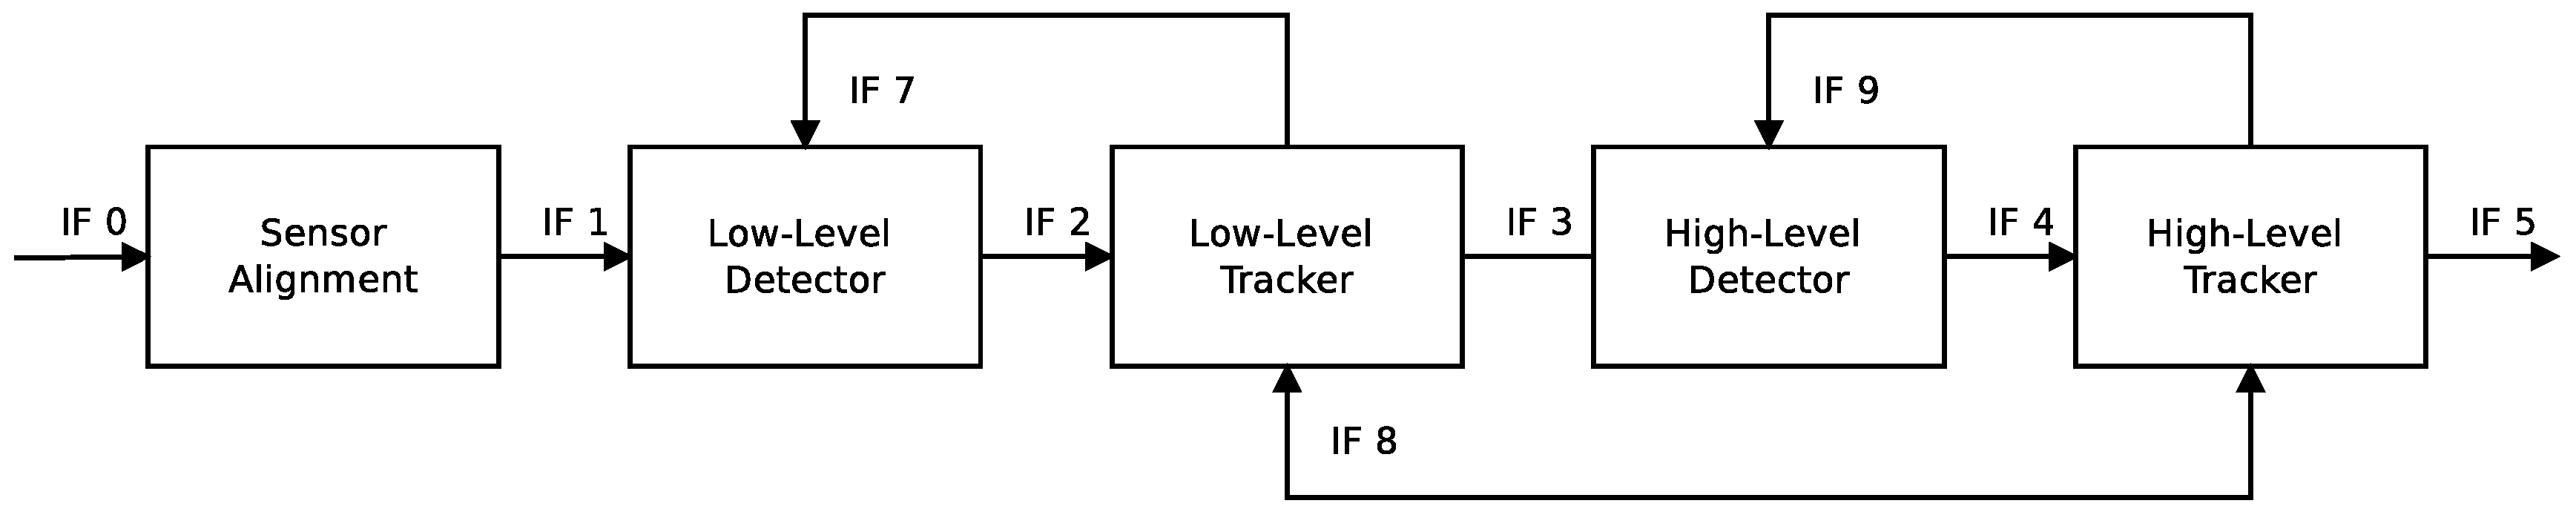
\includegraphics[width=\textwidth]{images/preliminary_design.eps}
\caption{Preliminary design.}
\label{fig:preliminary design}
\end{figure}

In the sequel, we describe the purpose of each component and what is being exchanged via each interface.
\begin{itemize}
\item The Sensor Alignment component applies the proper transformations to the Velodyne's raw measurements -- received via interface IF 0 -- to convert them from spherical to Cartesian coordinates including their corresponding covariance matrices. An unbiased transformation to accomplish this is presented in \cite{Barsh1}. The 3D Cartesian points and their covariance matrices are forwarded to the Low-Level Detector via interface IF 1;

\item The Low-Level Detector processes the aligned measurements to identify rectangular surfaces which may represent part of an observed vehicle. It delivers a set of detected rectangular surfaces\footnote{It is also necessary to model the uncertainty and randomness of this kind of measurement.} at the interface IF 2;

\item The Low-Level Tracker maintains a set of low-level tracks that represent rectangular surfaces being continuously tracked. It updates the low-level tracks based on the detects delivered at IF 2. The low-level tracks are forwarded to the High-Level Detector via the interface IF 3. Note that, despite not necessarily representing a moving object, a low level track is likely to represent a surface of a real obstacle in the world and could already be employed by the obstacle avoidance module. Moreover, the Low-Level Tracker may feedback the low-level tracks to the Low-Level Detector via interface IF 7 to help it pruning unlikely detects or direct its focus on specific areas on which it is more likely to detect rectangular surfaces;

\item The High-Level Detector identifies 3D boxes in the observed scenario based on the multiple low-level tracks being reported by the Low-Level Tracker via interface IF 3. More specifically, it identifies plausible combinations of the rectangular surfaces being tracked which are likely to represent a box shaped object in the observed scenario. It delivers the high-level detects at interface IF 4;

\item Finally, the High-Level Tracker maintains a set of high-level tracks that represent 3D boxes being tracked and, ultimately, the vehicles in the real world\footnote{We can use a simple Moving Target Indicator (MTI) procedure to discard stationary objects which are, in principle, already represented in the background occupancy grid map.}. It employs the high-level detects received via interface IF 4 to update the high-level tracks and delivers the final result at interface IF 5. Similarly to the Low-Level Tracker, the High-Level Tracker could feedback the boxes being tracked to the High-Level Detector via interface IF 9. Additionally, it could also feedback the high-level tracks to the Low-Level Tracker via interface IF 8. In special, the high-level tracks could be splitted into low-level tracks which are then inserted into the Low-Level Tracker. Next, the High-Level Tracker could directly update its tracks based on the corresponding low-level tracks, bypassing thus the High-Level Detector. Conversely, the Low-Level Tracker could employ long-term predictions produced by the High-Level Tracker to improve the measurement-to-track data association procedure performed at the low-level, i.e. the predicted high-level tracks are splitted into low-level tracks and then associated with low-level measurements. Note that the splitted high-level tracks will compete with existing low-level tracks for the low-level measurements during the data association process. Ultimately, if a high-level track consistently represents a object in the scenario, its corresponding low-level tracks will be more likely to associate with the low-level measurements and the competing tracks will be deleted due to starvation.
\end{itemize}

% ----------------------------------------------------------
% References
% ----------------------------------------------------------
\begin{thebibliography}{}
{
\bibitem{Barsh1} Y.~Bar-Shalom and X.~Li,
\newblock {\em Multitarget-Multisensor Tracking: Principles and Techniques.} YBS, Storrs, CT, 1995.

\bibitem{Mahler07} R.~P.~Mahler,
\newblock {\em Statistical Multisource-Multitarget Information Fusion.} Artech House Inc., Norwood, 2007.
}
\end{thebibliography}

% ----------------------------------------------------------
% End document
% ----------------------------------------------------------
\end{document}
